%source: HW09-Kashani

با رسم شکل موج، حداکثر فرکانس کاری مدار زیر را با درنظر گرفتن مفروضات زیر به‌دست آورید.

\begin{latin}
	Flip-Flop propagation delay = 5 ns\\
	Hold time = 3ns\\
	Setup time = 3ns\\
	XOR propagation delay = 2ns
\end{latin}


\begin{figure}[h]
	\centering
	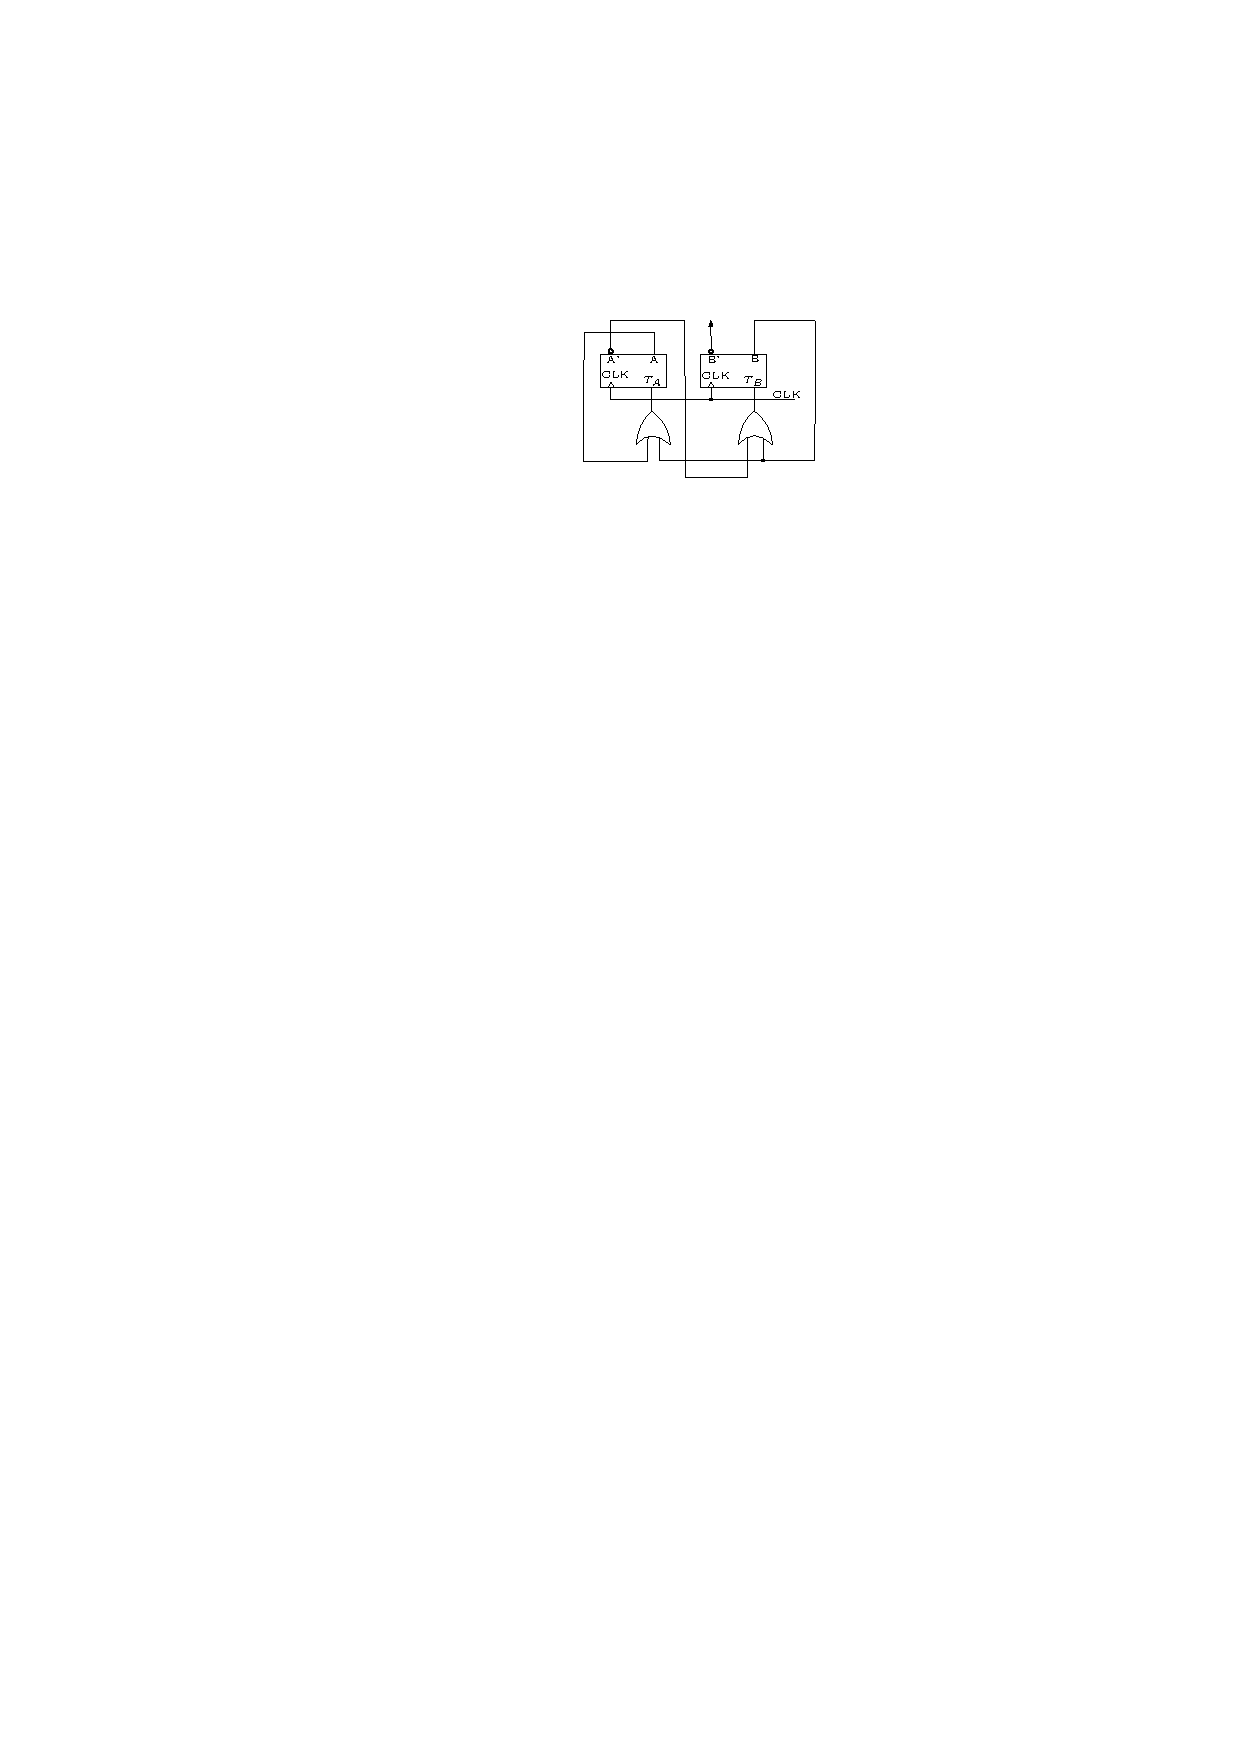
\includegraphics[width=0.4\textwidth]{fig/Q_basic7.pdf}
	\label{fig:Q_basic_7}
\end{figure}